\section{Addressing Emulation Attacks}
\label{sec:variantII}

We consider attestation key extraction from SGX processors difficult and rare, in contrast to the previously considered relay attacks that require only OS control or other malicious software on the target platform. However, the recently demonstrated Foreshadow attack~\cite{foreshadow-usenix18} that exploited the Meltdown vulnerability~\cite{Lipp2018meltdown} showed how to extract attestation keys from SGX processors. Although Intel has the possibility to issue microcode patches that address processor vulnerabilities like Meltdown and the processor's microcode version is reflected in the SGX attestation signature, new vulnerabilities like the ZombieLoad attack~\cite{ZombieLoad} may be discovered. Before microcode patches are deployed, in rare occasions, leaked but not revoked attestation keys may be available to the attacker.


\subsection{Addressing the Emulation Attack} 

\myparagraph{attacker model} 
We consider an \emph{emulation attacker} has all the capabilities of the relay attacker (cf.\ Section~\ref{sec:problemStatement}) and additionally has obtained at least one valid (not yet revoked by Intel) attestation key from any SGX platforms but the target platform. The attacker might obtain an attestation key by attacking one of his processors or by purchasing an extracted key from another party. 

\myparagraph{The emulation attack} 
In the attack, the attacker uses a leaked attestation key to emulate an SGX-processor on the target platform. Since the IAS (or any other attestation service) successfully attests to the emulated enclave, it is impossible for the remote verifier to distinguish between the emulated enclave and the real one. 


\myparagraph{Emulation attack implications} 
The emulation attack allows the attacker to fully control the attested execution environment and thus break the two fundamental security guarantees of SGX, enclave's data confidentiality and code integrity, and to access any secrets provisioned to the emulated enclave. Since the OS is also under the control of the attacker, any attempted communication with the real enclave will always be redirected to the emulated enclave.



\begin{figure}[t]
 \centering
%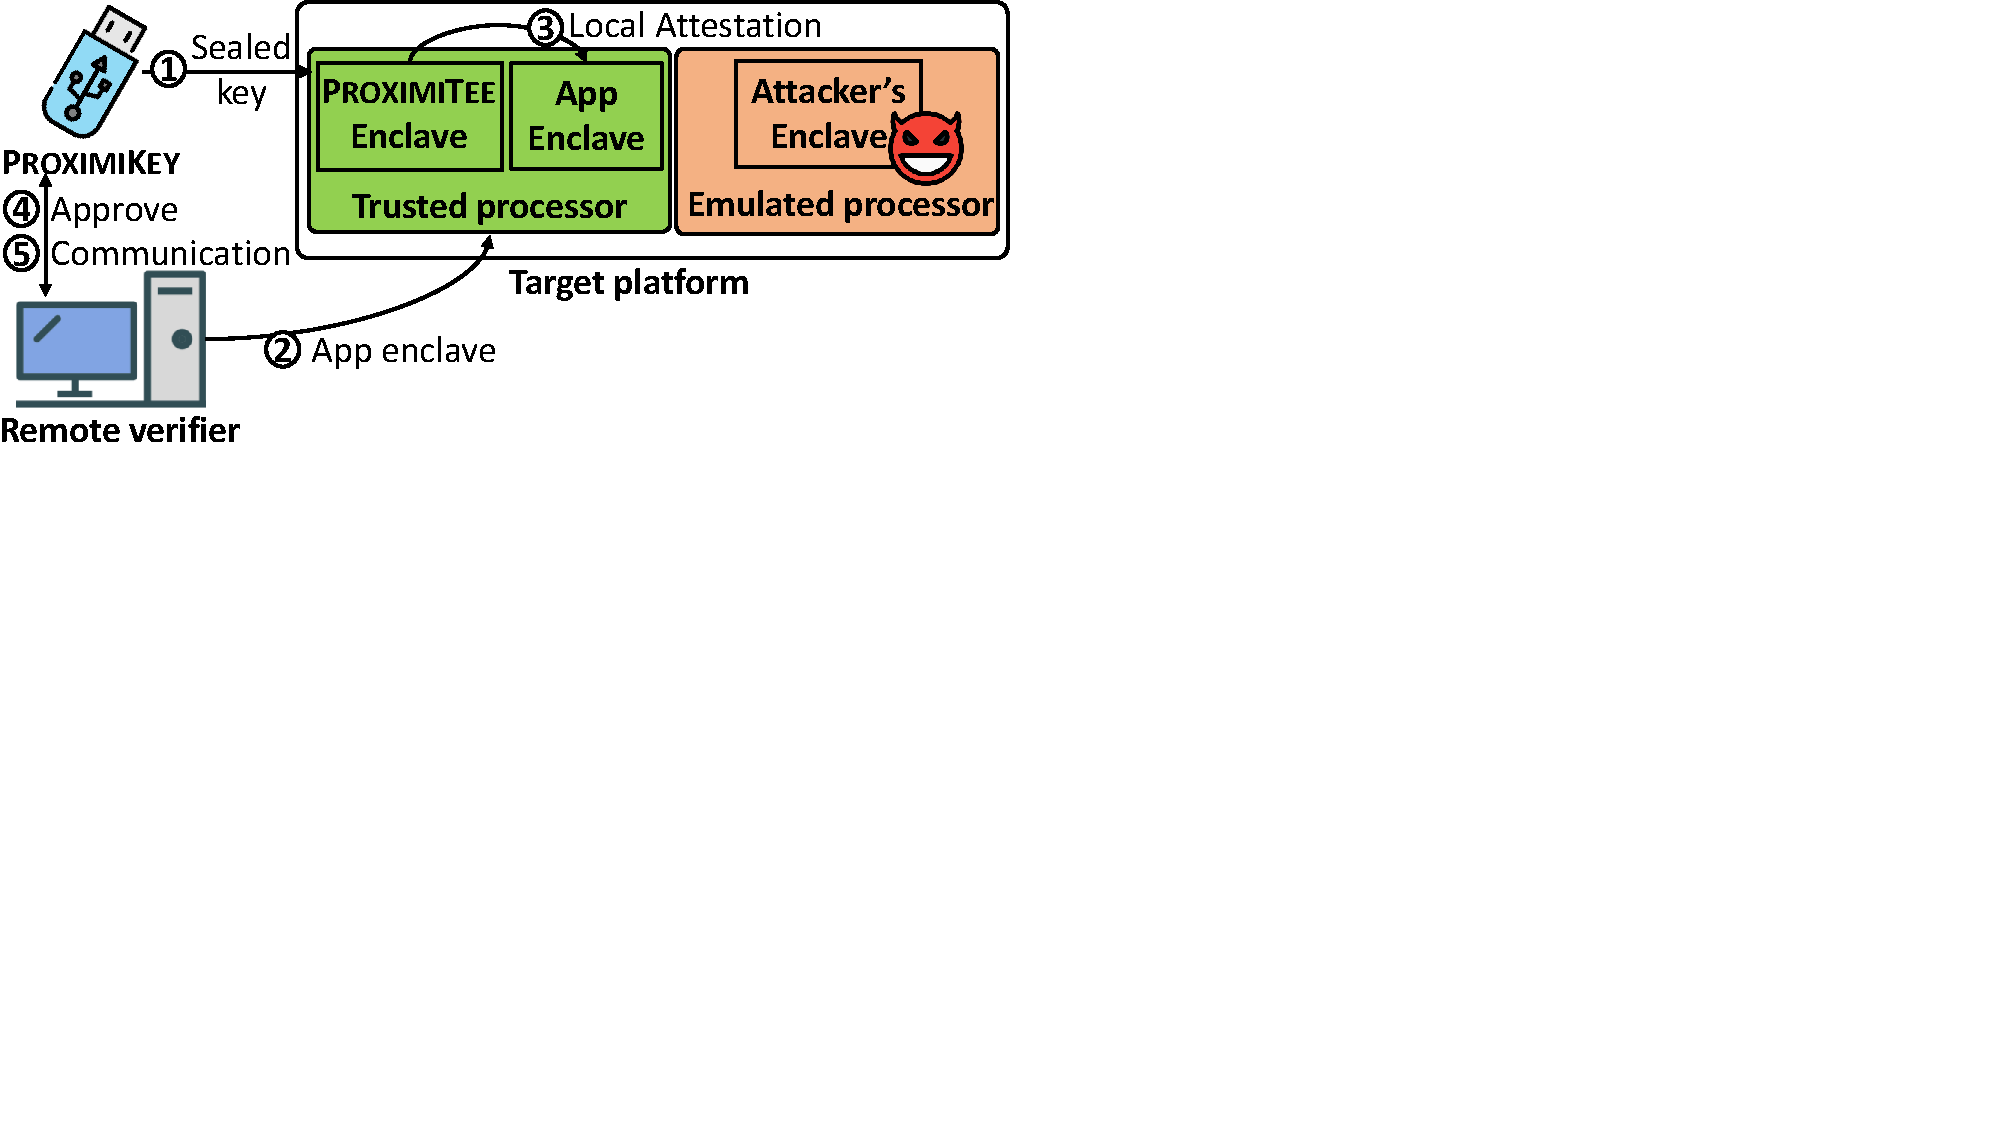
\includegraphics[trim={0 11.6cm 16.5cm 0},clip,width=0.72\linewidth]{chapters/ProximiTEE/figures/boot-attest.pdf}
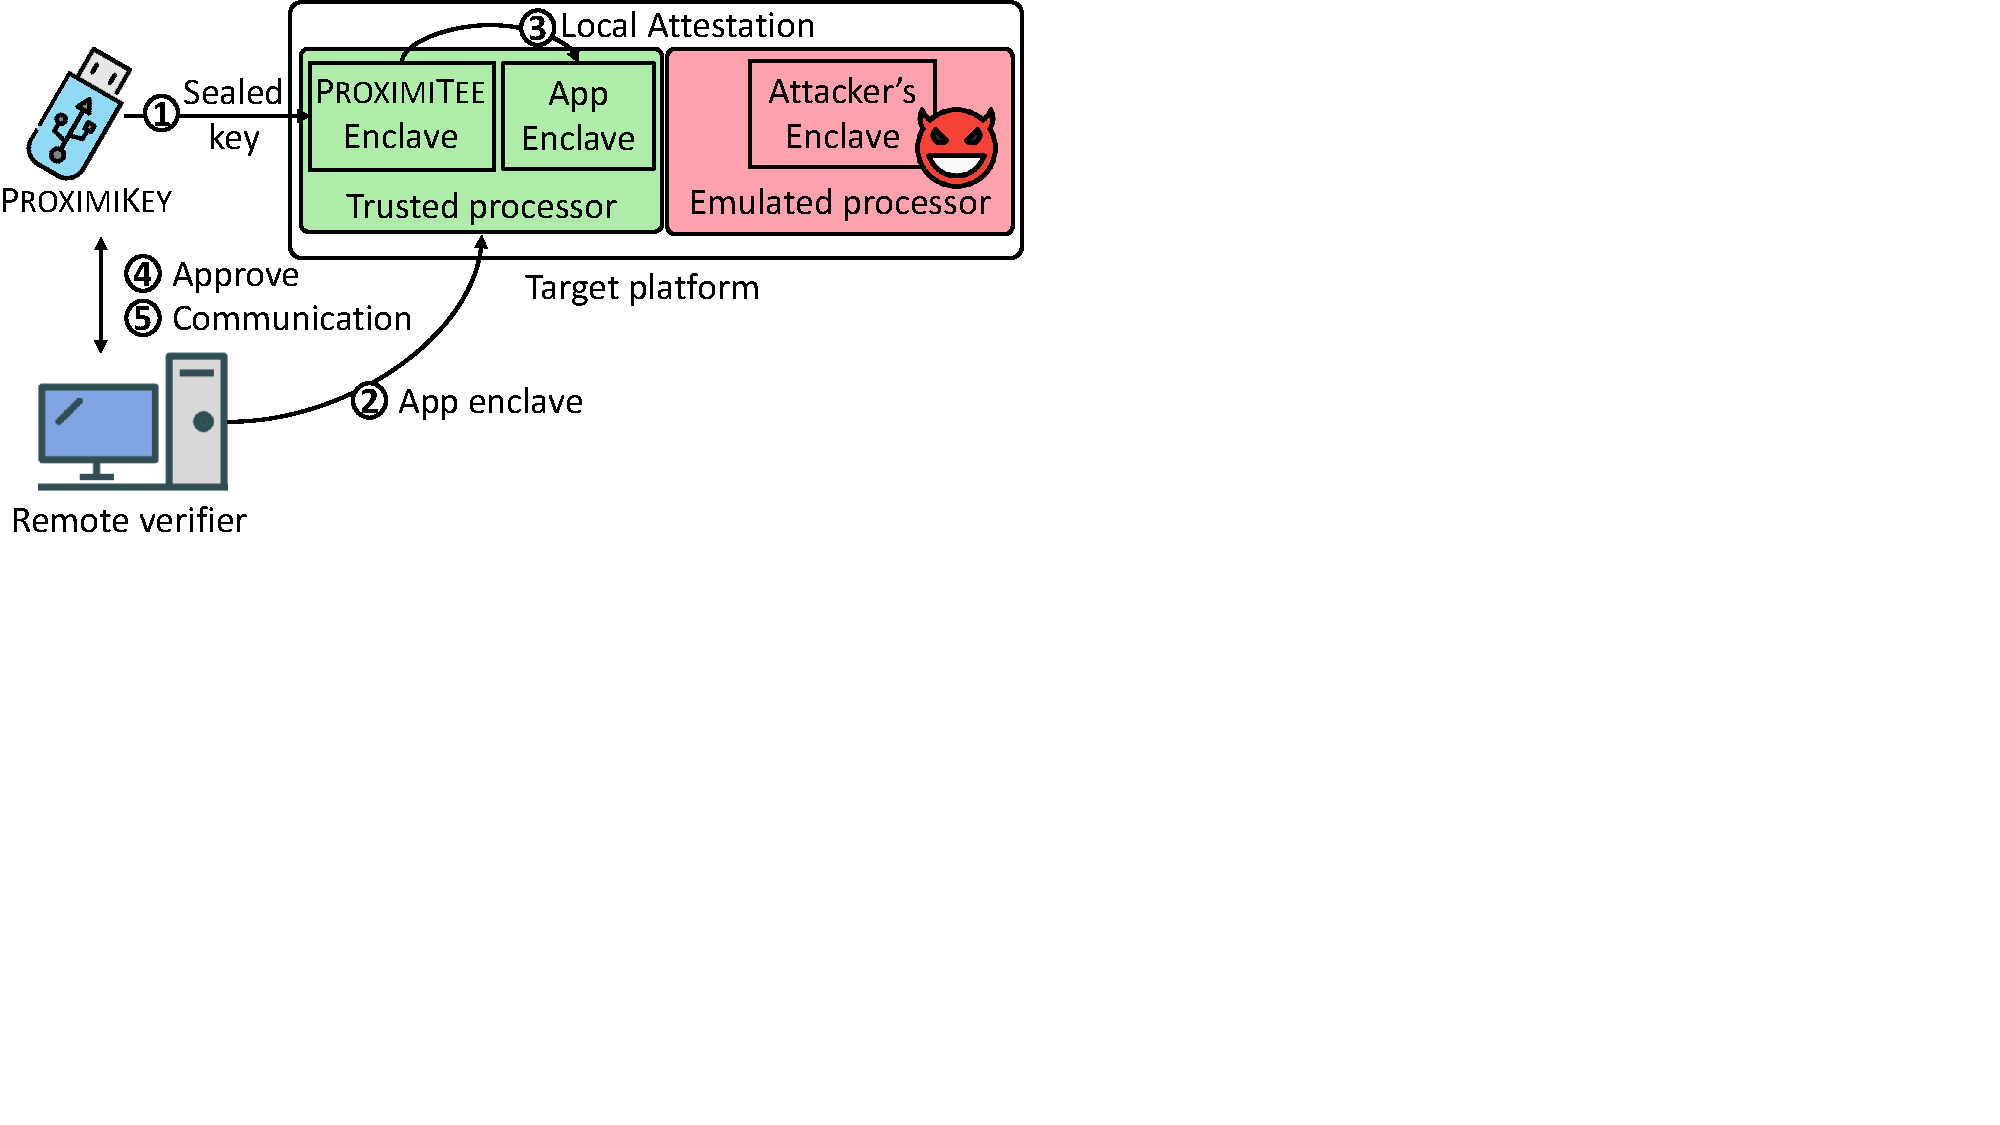
\includegraphics[trim={0 9cm 16.5cm 0},clip,width=0.72\linewidth]{chapters/ProximiTEE/images_new/boot_attest.pdf}
 \caption[\name boot-time attestation]{\textbf{\name boot-time attestation.} After the boot-time initialization (refer to Figure~\ref{fig:boot-init}) the \nameclave executes a local attestation with the verifier uploaded \app. 
 }
 \label{fig:boot-attest}
\end{figure}


\begin{figure}[t]
 \centering
    %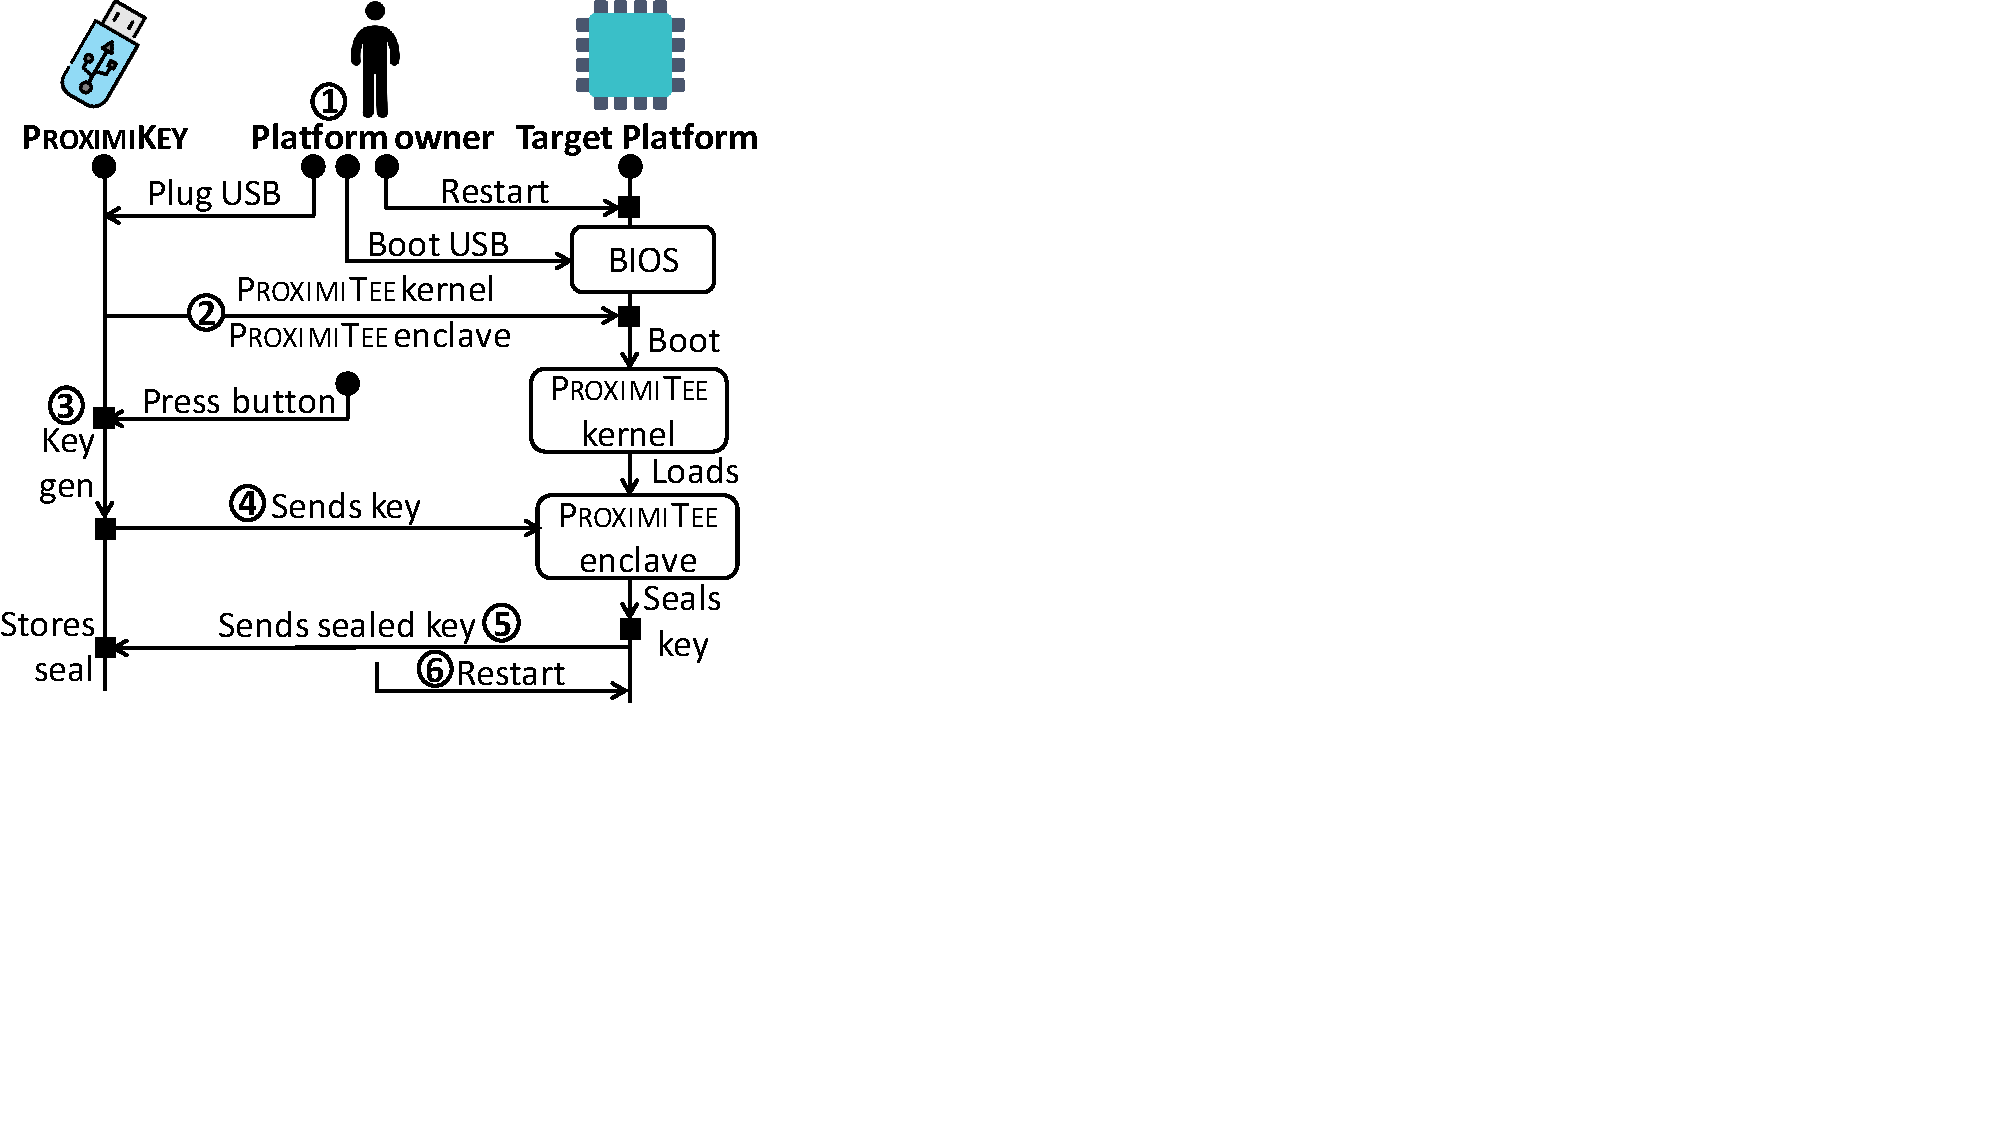
\includegraphics[trim={0 7cm 19cm 0},clip,width=0.7\linewidth]{chapters/ProximiTEE/figures/boot_init.pdf}
    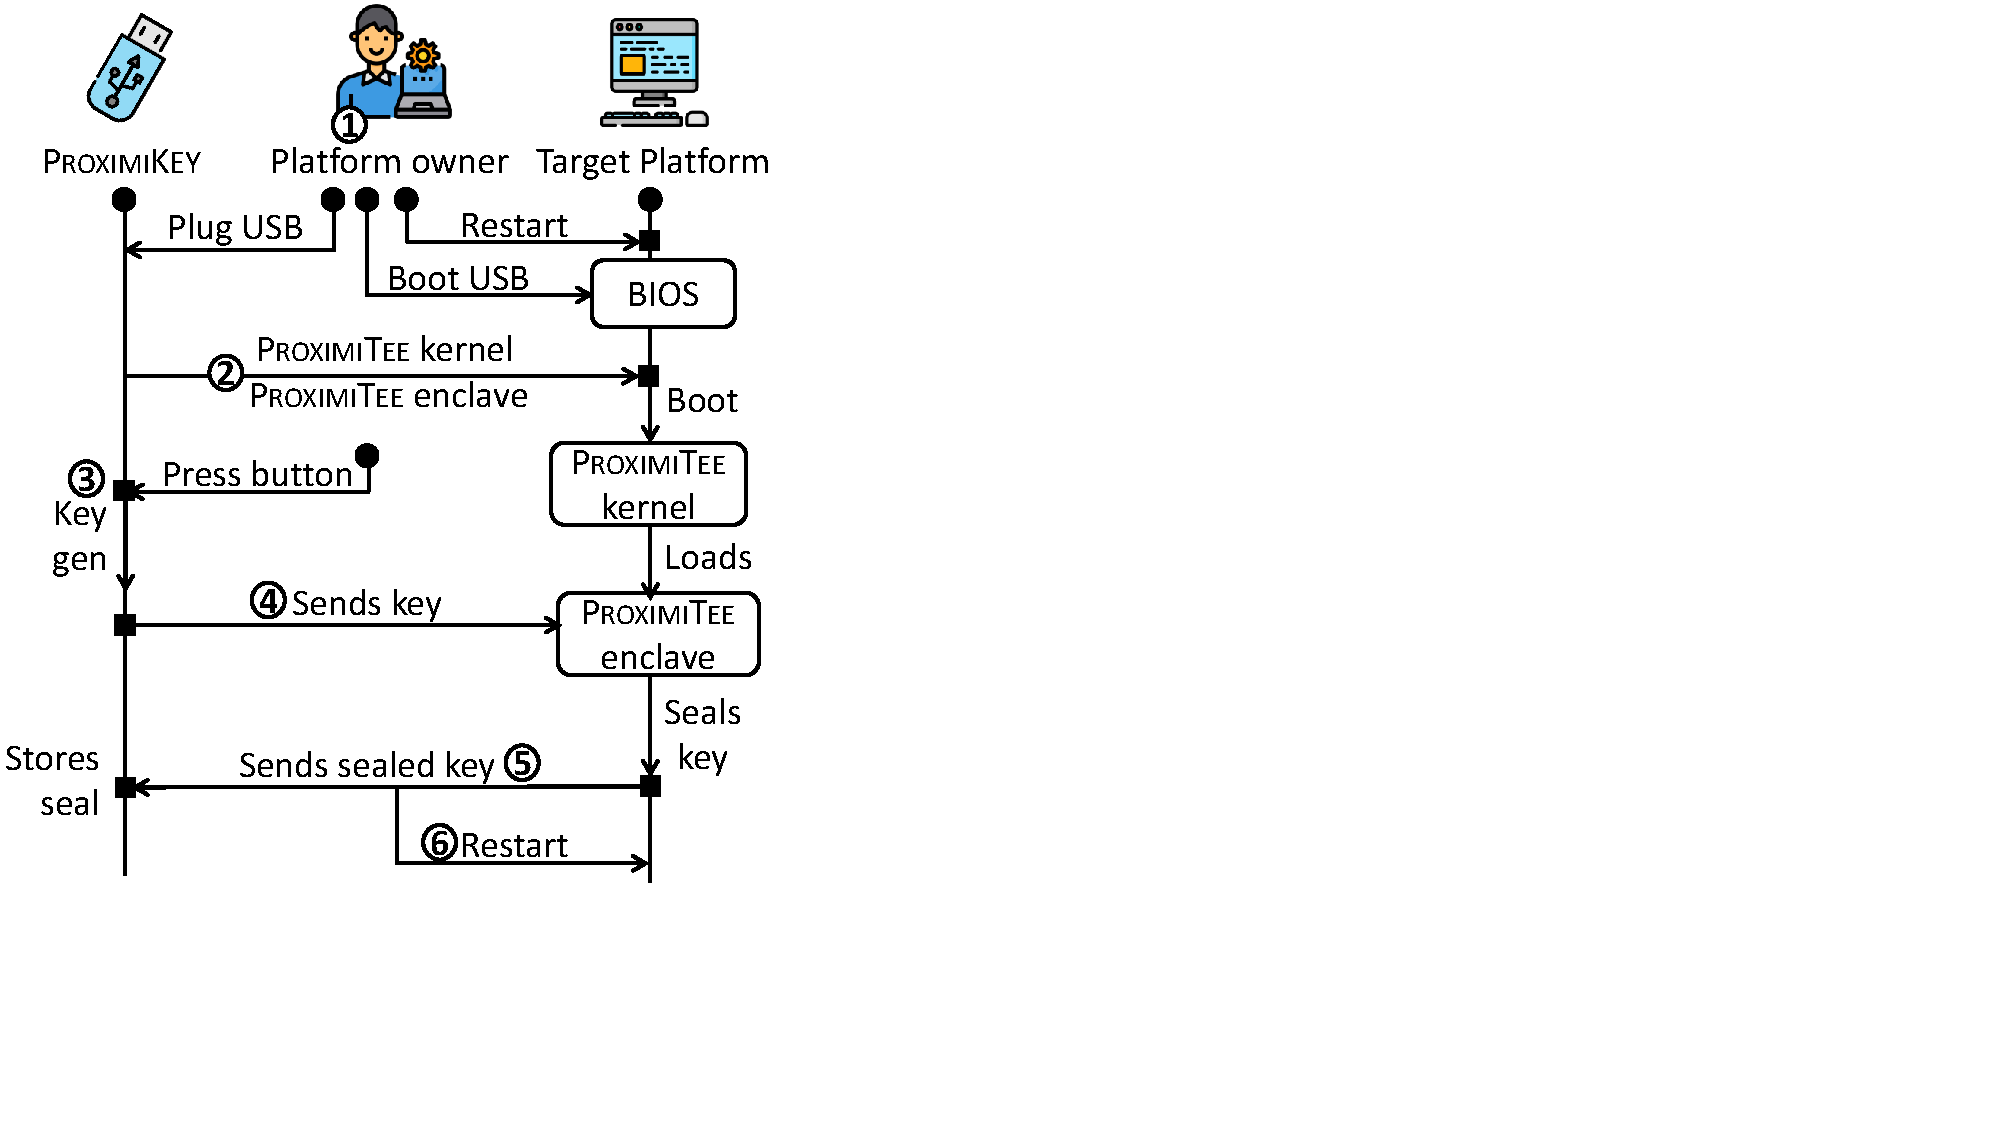
\includegraphics[trim={0 2cm 19cm 0},clip,width=0.7\linewidth]{chapters/ProximiTEE/images_new/boot_init.pdf}
 \caption[\name noot-time initialization]{\textbf{\name boot-time initialization.} The \device uses a minimal kernel Linux image to boot and load \nameclave on the target platform and seal a platform specific secret to the \device{}'s memory.}
 \label{fig:boot-init}
\end{figure}



\subsection{Boot-Time Initialization Solution}

Proximity verification alone cannot protect against the emulation attacker, as the locally emulated enclave would pass the proximity test. 
%
Therefore, we describe a second hardened attestation mechanism that leverages secure boot-time initialization and is designed to prevent emulation attacks. This solution can be seen as a \emph{novel variant} of the well-known TOFU principle, and the main benefit of our solution over previous variants is that it simplifies deployment and increases security. Additionally, when such attestation is used in combination with our previously described periodic proximity verification, our solution enables secure offline revocation.


\myparagraph{Security assumptions}
Our security assumptions regarding the target platform are as described in Section~\ref{sec:problemStatement}. The only difference is that in this case, we assume that the UEFI (or BIOS) on the target platform is trusted.


\myparagraph{Solution overview}
Figure~\ref{fig:boot-attest} illustrates an overview of this solution. During initialization, that is depicted in Figure~\ref{fig:boot-init}, the target platform is booted from the attached device that loads a minimal and single-purpose \name kernel on the target device. In particular, this kernel includes no network functionality. The kernel starts the \name enclave, which shares a secret with the device. This shared secret later bootstraps the secure communication between \device and the \name enclave. \emph{The security of the bootstrapping relies on the fact that the minimal kernel will not perform enclave emulation at boot time.} The \name enclave will later be used as a proxy to attest whether other (application-specific) enclaves in the system are real or emulated and on the same platform.


\myparagraph{Boot-time initialization} The boot-time initialization process is performed only once.
This process is depicted in Figure~\ref{fig:boot-init} and it proceeds as follows:


\begin{enumerate}
  \item[\one] The platform owner plugs \device to the target platform, restarts it to BIOS and selects the option to boot from \device.
  \item[\two] \device loads the \name kernel and boots from it. The \name kernel starts the \nameclave.
  \item[\three] The user presses a button on \device to confirm that this is a boot-initialization process. This step is necessary to prevent an attack where the compromised OS emulates a system boot.
  \item[\four] \device sends a randomly generated key $\mathcal{K}$ to the \nameclave.
  \item[\five] The enclave returns the sealed key $\mathcal{S}$ corresponding to the key $\mathcal{K}$ ($\mathcal{S}\leftarrow\texttt{Seal}(\mathcal{K})$) to \device that stores the key and the seal pair $(\mathcal{K}, \mathcal{S})$ on its flash storage.
  \item[\six] \device blocks further initializations, sends a restart signal and boots the platform with the normal OS.
\end{enumerate}


\myparagraph{Attestation process} After initialization the target platform runs a regular OS. The attestation process is depicted in Figure~\ref{fig:boot-attest} and proceeds as follows:

\begin{enumerate}


  \item[\one] \device sends the seal $\mathcal{S}$ to the \nameclave that unseals it and retrieves the key $\mathcal{K}$. \device and the \nameclave establish a secure channel (\tls) using $\mathcal{K}$.

  \item[\two] The remote verifier uploads a new \app on the target platform.

  \item[\three] The \nameclave performs local attestation (refer to~Section~\ref{ch:background:SGX:local}) on the \app that binds its public key to the attestation. %The local attestation ensures that i) the \app is on the same physical platform, and ii) the code integrity of the \app.

  \item[\four] The \nameclave sends the measurement and the public key of the \app to \device. \device establishes a secure channel to the \app and sends the measurement of the enclave to the remote verifier. The remote verifier then approves the communication to the \app.

  \item[\five] The remote verifier checks that the measurement of the \app is as expected. If this is the case, it can communicate with the enclave through \device.


\end{enumerate}


\myparagraph{Following communication} 
Similar to our previous solution, after the initial attestation, all the communication between a remote verifier and the enclave is mediated by the \device that periodically checks the proximity of the attested enclave and terminates the communication channel in case the embedded device is detached.


\subsection{Security Analysis and Implementation}
 
In this attestation mechanism, the task of establishing a secure communication channel to the correct enclave can be broken into three subtasks. The first subtask is to establish a secure channel to the correct \device device. In our solution, this is achieved using standard device certification. Recall that the attacker cannot compromise the specific \device used. 

The second subtask is to establish a secure communication channel from \device to the \nameclave. \device shares a key with an enclave that is started by the trusted \name kernel, hence at a time in which the attacker could not emulate any enclave. \device knows when secure initialization takes place as the platform owner indicates this by pressing a button -- an operation that the attacker cannot perform. The \nameclave seals the key during initialization. Different SGX CPUs cannot unseal each other's data, and therefore even if the attacker has extracted sealing keys from other SGX processors, she cannot unseal the key and masquerade as the legitimate \nameclave. 

The third subtask is to establish a secure communication channel from the \nameclave to the \app. The security of this step relies on SGX's built-in local attestation. An attacker in possession of leaked sealing attestation keys from other SGX processors cannot produce a local attestation report that the \name enclave would accept, and therefore the attacker cannot trick the remote verifier into establishing a secure communication channel to a wrong enclave.


\myparagraph{Comparison to TOFU} Our second attestation mechanism is a novel variant of the well-known ``trust on first use'' principle. In this section, we briefly explain the main benefits of our solution over common TOFU variants. 

\begin{enumerate}
\item \emph{Smaller TCB size and attack surface.} 
In the TOFU solution, the standard and general-purpose OS needs to be trusted on first use, and the CA needs to remain online for enrollment of new SGX platforms. In our solution, a significantly smaller and single-purpose kernel needs to be trusted on first use. Additionally, we require trust in the BIOS (or UEFI). In our solution, the CA can remain offline when a new platform is enrolled.


\item \emph{Reboot instead of reinstall.} Our solution requires that the target platform is rebooted once from \device. In most TOFU solutions, the target platform requires a clean state which is difficult to achieve without reinstall that makes deployment difficult.


\item \emph{Secure offline revocation.} When boot-time initialization is combined with the previously explained periodic proximity verification, our solution provides an additional property of secure offline revocation that requires no interaction with the CA. Such property is missing from previous TOFU solutions.

\end{enumerate}

\myparagraph{Implementation} We implemented a complete prototype of our second attestation mechanism. On top of our previous \name implementation (refer to Section~\ref{sec:implementation}), the boot-time initialization solution requires the \name kernel. We have modified an image of Tiny Core Linux~\cite{tinyCore} and used it as the boot image for our boot-time initialization. The image size of our modified Linux distribution is 14 MB (in contrast to 2 GB standard 64 bit Linux images build on the standard kernel). Our image supports bare minimum functionality and includes \texttt{libusb}, \texttt{gcc}, Intel SGX SDK, Intel SGX platform software (PSW), and Intel SGX Linux driver. The \name enclave is a minimal enclave that uses a simple serial library to communicate with the \device and local attestation mechanism to attest any application-specific enclave.
